\documentclass[paper=a4, fontsize=11pt]{scrartcl}
\usepackage[T1]{fontenc}
\usepackage[utf8]{inputenc}
\usepackage{lmodern}
\usepackage{multirow}
\usepackage[table,xcdraw]{xcolor}
\usepackage[spanish]{babel}
\usepackage{cite}
\usepackage{amsmath,amsfonts,amsthm} % Math packages
\usepackage{graphics,graphicx, float} %para incluir imágenes y colocarlas
\usepackage[backref,colorlinks=true,linkcolor=black,urlcolor=blue,citecolor=blue]{hyperref} %Para crear enlaces en el pdf
\usepackage[noabbrev,spanish]{cleveref}
\usepackage{url}
\usepackage[shortlabels]{enumitem}
\usepackage{appendix}
\usepackage{eurosym}
\usepackage{epsfig}
\usepackage{caption}
\usepackage{subcaption}

\renewcommand{\appendixname}{Anexo}
\renewcommand{\appendixtocname}{Anexo}
\renewcommand{\appendixpagename}{Anexo}

\numberwithin{figure}{section} % Number figures within sections (i.e. 1.1, 1.2, 2.1, 2.2 instead of 1, 2, 3, 4)
\numberwithin{table}{section} % Number tables within sections (i.e. 1.1, 1.2, 2.1, 2.2 instead of 1, 2, 3, 4)
\newcommand{\horrule}[1]{\rule{\linewidth}{#1}} % Create horizontal rule command with 1 argument of height

\title{
    \normalfont \normalsize
    \textsc{{\bf Ingeniería de Servidores (2015-2016)} \\ Grado en Ingeniería Informática \\ Universidad de Granada} \\ [25pt] % Your university, school and/or department name(s)
    \horrule{0.5pt} \\[0.4cm] % Thin top horizontal rule
    \huge Memoria Práctica 5 \\ % The assignment title
    \horrule{2pt} \\[0.5cm] % Thick bottom horizontal rule
}
\author{Antonio de la Vega Jiménez }

%*************************************************************


\begin{document}

\maketitle % Muestra el Título
\newpage %inserta un salto de página
\tableofcontents % para generar el índice de contenidos
\listoffigures
\listoftables
\newpage

%*************************************************************
\section{Concepto de máquina virtual y virtualización}
\subsection{Cuestión 1} 
\textit{¿Qué modos y/o tipos de “virtualización” existen? } \newline 

Existen tres tipos principales de virtualización: Paravirtualización, virtualización por hardware  y virtualización por hardware con drivers paravirtualizados.


\begin{itemize}
    \item \textbf{Paravirtualización:} En este modo el kernel del SO huésped es modificado ( remplazando las instrucciones no virtualizables con ``hypercalls'' que se comunican directamente con el hipervisor),
de este modo el SO huésped es capaz de ejecutarse a una velocidad similar a la de la ejecución nativa. Este tipo de virtualización presenta dos problemas, la modificación del SO es complicada y puede hacer difícil su mantenimiento, además, los sistemas operativos no modificables como Windows XP no son soportados. \cite{vmware} \cite{vmoracle} 
    
    \item \textbf{Virtualización por hardware o virtualización completa:} En este caso no se necesita ninguna modificación del SO, pero si es necesario que exista soporte para la virtualización por hardware(Intel VT o AMD-V). Con la implementación actual pueden existir algunas penalizaciones de rendimiento en ciertos tipos de huéspedes y tipos de accesos, aunque posee la ventaja de ser compatible con un mayor numero de sistemas operativos. \cite{vmoracle}
    
    \item \textbf{Virtualización por hardware con drivers paravirtualizados:} Este tipo es igual a la virtualización por hardware, pero con una serie de drivers paravirtualizados añadidos que sirven para mejorar la eficiencia de la máquina virtual.\cite{vmoracle}
\end{itemize}


\subsection{Cuestión 2}
\textit{Muestre los precios y características de varios proveedores de VPS (Virtual Private Server) y compare con el precio de servidores dedicados (administrados y no administrados). Comente diferencias}. \newline

En la siguiente tabla ( Tabla \ref{Tabla1}) se muestra una comparación de las características ofrecidas por varios proveedores de VPS en un rango de precio similar, y en la Tabla \ref{Tabla2}, se muestra una comparativa de servidores dedicados:
\newpage

\begin{table}[h]

\resizebox{17 cm}{!}{
\hskip-2.2cm
\begin{tabular}{|
>{\columncolor[HTML]{C0C0C0}}l |c|c|c|c|}
\hline
{\color[HTML]{000000} Proveedor}      & \cellcolor[HTML]{EFEFEF}Hostinger - Plan 4 & \cellcolor[HTML]{EFEFEF}OVH - VPS CLOUD 3 & \cellcolor[HTML]{EFEFEF}gigas - VPS pro & \cellcolor[HTML]{EFEFEF}Strato - VPS Linux L3 \\ \hline
{\color[HTML]{000000} Precio}         & 27,99 \euro                               & 29,99 \euro                               & 29 \euro                              & 24,90 \euro                                       \\ \hline
{\color[HTML]{000000} RAM}            & 4GB Garantizada / 8GB Dinámica             & 8GB                                       & 4GB                                     & Hasta 16GB                                    \\ \hline
{\color[HTML]{000000} Cores}          & 2 - 4                                      & 4                                         & 4                                       & 8                                             \\ \hline
{\color[HTML]{000000} Almacenamiento} & 60GB                                       & 100GB                                     & 50GB                                    & 600GB                                         \\ \hline
\end{tabular}
}
\caption{Comparativa proveedores VPS }
\advance\leftskip 5cm
Fuentes: \cite{vps1} \cite{vps2} \cite{vps3} \cite{vps4}
\label{Tabla1}
\end{table}


\begin{table}[h]

\resizebox{17 cm}{!}{
\hskip-2cm
\begin{tabular}{|
>{\columncolor[HTML]{C0C0C0}}l |c|c|c|}
\hline
{\color[HTML]{000000} Proveedor} & \cellcolor[HTML]{EFEFEF} Strato \newline Servidor Dedicado Linux Level 1 & \cellcolor[HTML]{EFEFEF}OVH - HOST-32L & \cellcolor[HTML]{EFEFEF}Hostalia - Dell PowerEdge R220          \\ \hline
{\color[HTML]{000000} Precio}         & 29 \euro                                  & 59,99 \euro                                                                       & 69,90 \euro                                   \\ \hline
{\color[HTML]{000000} RAM}            & 4 GB                                     & 32 GB                                                                              &  16GB                                           \\ \hline
{\color[HTML]{000000} Procesador}     & AMD Opteron 1214 HE                      & Intel Xeon D-1520                                                                  &1 x E3-1241 v3                                   \\ \hline
{\color[HTML]{000000} Almacenamiento} & 2x500 GB                                 & 2x2TB                                                                        & 2x1TB                                                 \\ \hline
{\color[HTML]{000000} Modelo } &    -                                            & -                                                                           & Dell PowerEdge R220                                    \\ \hline

\end{tabular}
}
\caption{Comparativa proveedores servidores dedicados. }
\advance\leftskip 5cm
Fuentes: \cite{serv1} \cite{serv2} \cite{serv3} 
\label{Tabla2}
\end{table}

Una de las principales diferencias es que en los servidores dedicados te especifican el modelo del procesador, el tipo de RAM, el numero de discos duros..., otra diferencia importante es que en los servidores VPS se pueden encontrar precios más económicos que en los servidores dedicados, esto puede deberse a que en el caso de los servidores VPS un servidor puede ser ``repartido'' entre varios clientes, mientras que en un servidor dedicado tienes que alquilarlo al completo.



\subsection{Cuestión 3} 

\textit{¿Qué otros software de virtualización existen además de VMWare y VirtualBox?} \newline

Además de  VMWare y VirtualBox existen otros software de virtualización, algunos ejemplos son:
\begin{enumerate}
    \item Quemu \cite{quemu}
    \item Parallels \cite{parallels}
    \item Proxmox \cite{proxmox}
    \item Xen \cite{xen}
\end{enumerate}

%*************************************************************
\section{Instalación de sistemas operativos virtualizados}
\subsection{Introducción}
\subsubsection{Cuestión 4}
\textit{Enumere algunas de las innovaciones en Windows 2012 R2 respecto a 2008 R2.} \newline

Existen numerosas innovaciones en la version 2012 R2 de Windows server respecto a la version 2008 R2, algunas de ellas son:

Un host con Windows Server 2012 R2 soporta 320 procesadores lógicos , 4TB de memoria RAM y 2048 procesadores virtuales por host, mientras que Windows Server 2008 R2 soporta 64 procesadores lógicos, 1TB de memoria y 512 procesadores virtuales por host. También existen claras diferencias en sus características para maquinas virtuales y clúster, con Windows Server 2012 R2 una maquina virtual puede tener una capacidad de disco virtual de 64TB y pueden existir 1024 maquinas virtuales activas, mientras que en Windows Server 2008 R2 el disco duro virtual tiene una capacidad máxima de 2TB y pueden existir hasta 384 maquinas virtuales activas, respecto a los clúster en la versión de 2008 podían existir 16 nodos y hasta 1000 maquinas virtuales, en la nueva versión ( Windows Server 2012 R2 ) un clúster puede tener 64 nodos y hasta 8000 maquinas virtuales. Además de estas diferencias existen otras que se pueden consultar en la pagina web de Microsoft. \cite{2008vs2012}


\subsubsection{Cuestión 5}
\textit{¿Qué empresa hay detrás de Ubuntu? ¿Qué otros productos/servicios ofrece?} \newline

La empresa que hay detras de Ubuntu es Canonical. \cite{canonical}
El principal servicio de Canonical es Ubuntu Advantage, un servicio para Ubuntu, que consiste en la administración de servidores, plataformas cloud... \cite{canonical1}
Ademas de este servicio, dispone de otros, como son: GNU Bazaar, Storm, Juju, Upstart, Launchpad y Ubuntu Software Center.\cite{canonical2}

\subsubsection{Cuestión 6}
\textit{¿Qué relación tiene esta distribución(CentOS) con Red Hat y con el
proyecto Fedora?} \newline

CentOS está construido a partir del código fuente público de RedHat, además RedHat está proporcionando ayuda para crear una estructura para dirigir el proyecto CentOS ( ya que RedHat tiene más experiencia como empresa ) y algunos miembros de CentOS trabajan para RedHat, es decir CentOS y RedHat han unido sus fuerzas para conseguir un desarrollo mejor y más rápido. Por otro lado está el proyecto Fedora, que es un proyecto de código abierto y totalmente gratuito soportado por RedHat, las innovaciones llevadas a cabo en este proyecto son llevadas a RedHat y en consecuencia a CentOS. En resumen las tres distribuciones forman un gran grupo con el fin de mejorar mas rápido. \cite{fcentos} \cite{redhat1} \cite{redhat2}

\subsubsection{Cuestión 7}
\textit{Indique qué otros SO se utilizan en servidores y el porcentaje de uso (no olvide poner la fuente de donde saca la información y preste atención a la fecha de ésta).} \newline

\begin{table}[h]
\hskip -0.5cm
    \begin{tabular}{|c|c|c|c|c|c|c|}
        \hline
        \multicolumn{6}{|c|}{UNIX 67,2\%}                                                  & \multicolumn{1}{l|}{Microsoft Windows} \\ \hline
        Linux  & BSD   & Darwin          & HP-UX           & Solaris         & Desconocido & \multirow{2}{*}{32,8\%}                \\ \cline{1-6}
        53.1\% & 1.3\% & \textless 0.1\% & \textless 0.1\% & \textless 0.1\% & 45.5\%      &                                        \\ \hline
    \end{tabular}
    \label{Tabla3}
    \caption{Tabla porcentaje de uso de los SO en servidores }
    Nota: OS X Server no se muestra porque esta usado en menos de un 0,1\% de los servidores.\cite{serv1} \cite{serv2}
\end{table}


\begin{table}[h]
\centering
\begin{tabular}{|c|c|}
\hline
Distribucion     & \% uso          \\ \hline
Debian           & 31.7\%          \\ \hline
Ubuntu           & 29.8\%          \\ \hline
CentOS           & 20.7\%          \\ \hline
Red Hat          & 4.3\%           \\ \hline
Gentoo           & 2.1\%           \\ \hline
Fedora           & 1.3\%           \\ \hline
SuSE             & 1.1\%           \\ \hline
Scientific Linux & 0.1\%           \\ \hline
Turbolinux       & 0.1\%           \\ \hline
Mandriva         & 0.1\%           \\ \hline
CloudLinux       & \textless 0.1\% \\ \hline
Asianux          & \textless 0.1\% \\ \hline
Mageia           & \textless 0.1\% \\ \hline
StartCom Linux   & \textless 0.1\% \\ \hline
PLD Linux        & \textless 0.1\% \\ \hline
Unknown          & 8.7\%           \\ \hline
\end{tabular}
\caption{Porcentaje de uso de cada distribución en el 53.1\% de Linux  }
Fuente:\cite{serv3}
\label{Tabla4}
\end{table}

\subsection{Linux: Particionamiento del disco duro virtual y creación de RAID1}
\subsubsection{Cuestión 8}
\textit{¿Qué diferencia hay entre RAID mediante SW y mediante HW?} \newline

El objetivo de un RAID es visualizar múltiples discos duros independientes como si solo fuera uno, con el fin de mejorar el rendimiento, la capacidad y la fiabilidad. Un RAID se puede implementar mediante software o mediante hardware.

En un RAID hardware se necesita un soporte hardware en el que se conectan los discos, este soporte posee un controlador que se encarga de realizar las operaciones asociadas al RAID, este RAID se conecta al host de forma normal, de modo que para el host parece un solo disco y no requiere ninguna sobrecarga.

Por otro lado existen los RAID software, en este caso no es necesario hardware adicional y en consecuencia tiene la ventaja de no tener coste alguno. En un RAID software las operaciones relacionadas con este, son ejecutadas por la CPU del host, añadiendo una sobrecarga. Este tipo de RAID puede presentar algunas desventajas, como un rendimiento inferior, aunque con la capacidad de procesamiento de las CPUs actuales en algunos casos puede superar al rendimiento de un RAID hardware. \cite{raid1} \cite{raid2}

\subsubsection{Cuestión 9}
\textit{a) ¿Qué es LVM? b)¿Qué ventaja tiene para un servidor de gama baja? c) Si va a tener un servidor web, ¿le daría un tamaño grande o pequeño a /var?} \newline
\begin{enumerate}[a)]
    \item LVM es una herramienta para la administración de volúmenes lógicos que proporciona una abstracción ( una vista independiente del hardware ) del almacenamiento, dándole al administrador una mayor flexibilidad para asignar espacio, redimensionar volúmenes o para combinar varios volúmenes físicos en uno. También permite crear Snapshots de forma más eficiente.  \cite{lvm1} \cite{lvm2}
    \item Tiene la ventaja de que el tamaño de los volúmenes puede ser cambiado sin necesidad de formatear por lo tanto es más fácil aprovechar al máximo la capacidad del disco, por ejemplo en caso de haber calculado mal el espacio necesario para / de forma que queda sitio sin usar, este espacio desperdiciado se puede pasar a otra partición como /home o en caso de llenarse la partición / se le podría dar espacio de la partición /home si tener que formatear el disco de nuevo, además sería se puede aumentar la capacidad de almacenamiento del servidor sin tener que formatear nada. \cite{lvm3}
    \item Debería tener un tamaño grande, ya que en este directorio (/var) se almacenan las web.
\end{enumerate}

\subsubsection{Cuestión 10}
\textit{¿Debemos cifrar también el volumen que contiene el espacio para swap? ¿y el volumen en el que montaremos /boot?} \newline

La partición swap sí debe estar cifrada, ya que si no es así el cifrado de las otras particiones podría ser inútil. Por ejemplo, puede existir una aplicación que guarda archivos de contraseñas, en principio todo esta cifrado, pero cuando esta aplicación es pasada a memoria principal es descifrada, luego la aplicación puede ser pasada a swap copiando las contraseñas descifradas al disco (en caso de que el volumen que contiene swap no este cifrado), de manera que la información ya no estaría protegida y podría ser accedida desde otro programa. \cite{swap} Además en caso de no cifrarla y sí cifrar las demás, el instalador da un error como se puede ver en la Figura \ref{fig1}

El volumen /boot no tenemos por que cifrarlo, ya que no contiene información crítica(y además si lo ciframos no podría arrancar el sistema ya que no dispongo de las herramientas necesarias), aunque en caso de ser necesario se puede cifrar. \cite{boot}

\begin{figure}[H]
    \begin{center}
        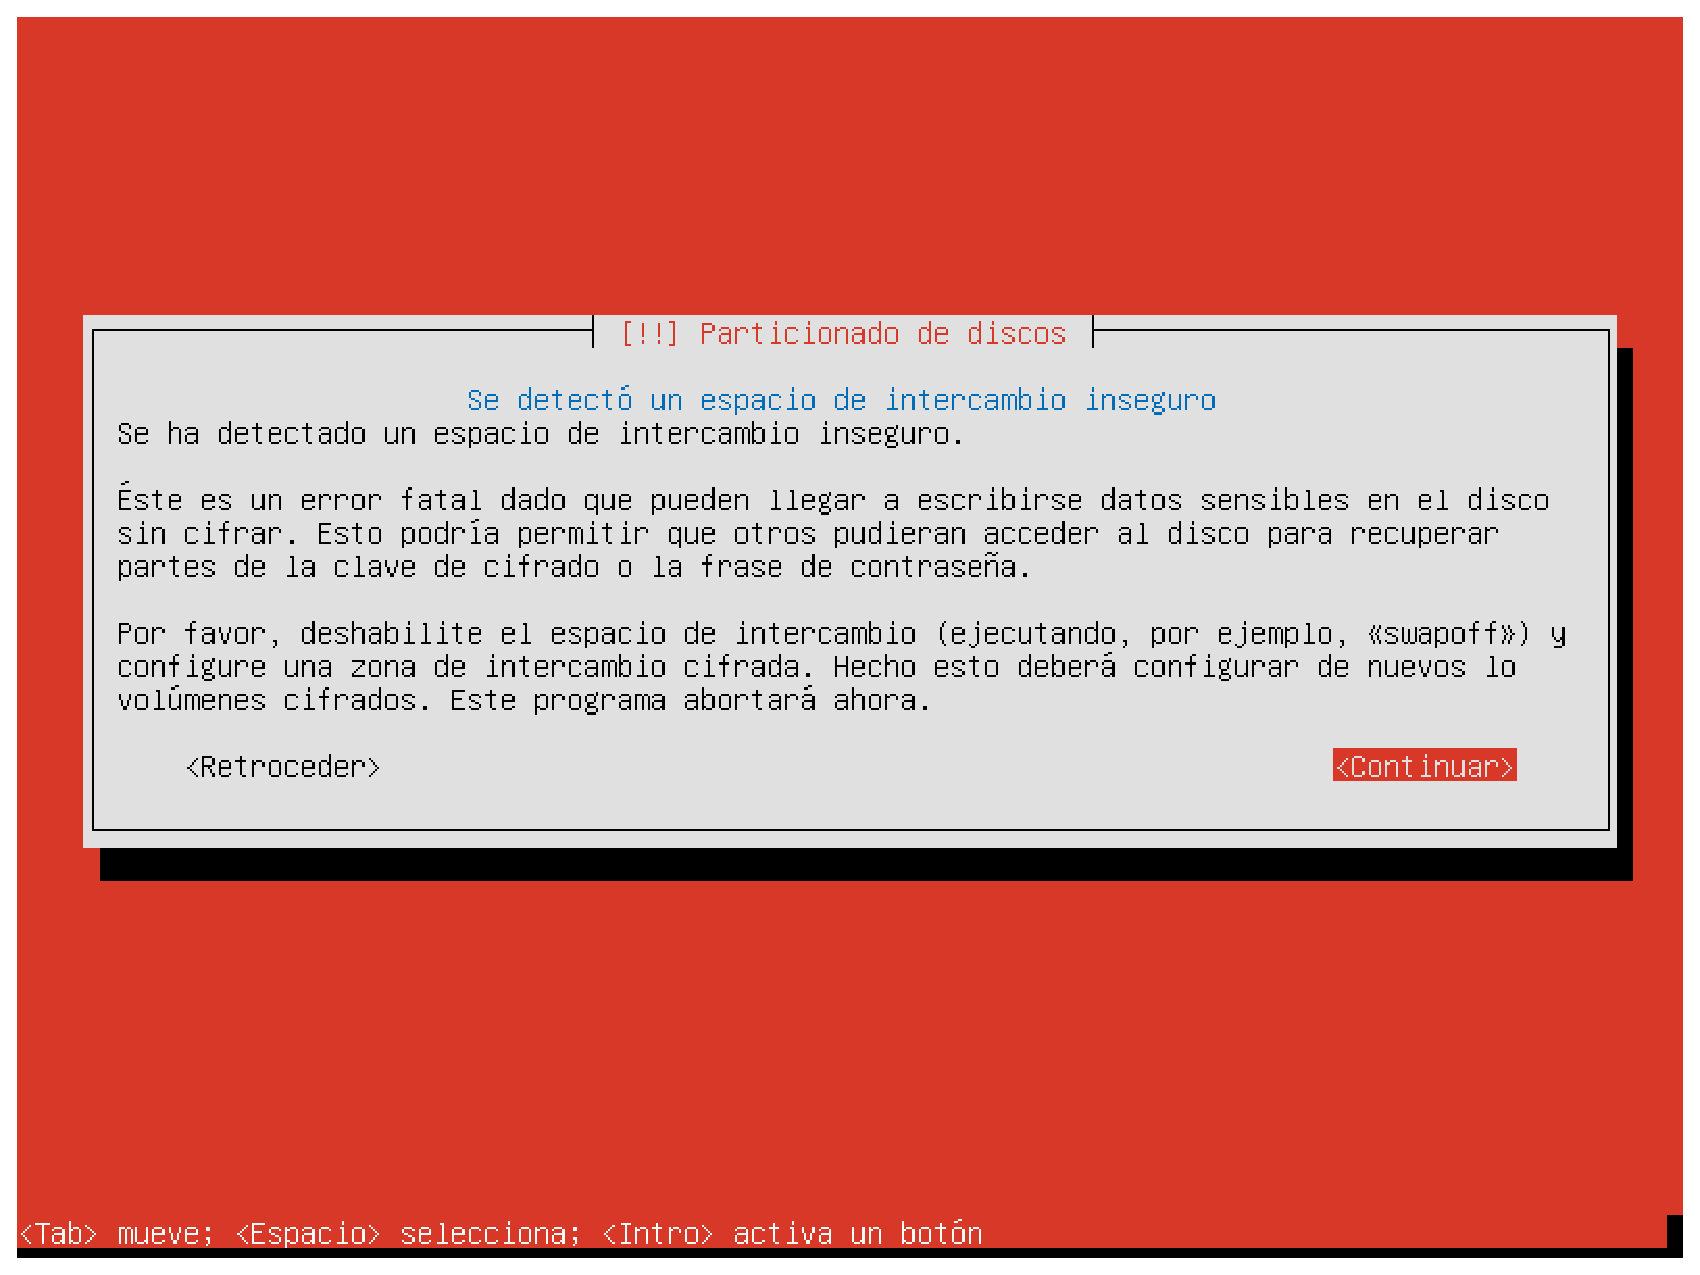
\includegraphics[scale=0.4]{Imagenes/swap_sin_cifrar.eps}
        \caption{Error lanzado por el instalador cuando la partición swap no está cifrada.}
        \label{fig1}
    \end{center}
\end{figure}

\subsubsection{Cuestión 11}
\textit{¿Qué otro tipo de usos de una partición le permite configurar el asistente de instalación? ¿Cuál es la principal diferencia entre ext4 y ext2?} \newline

Los posibles usos que se permiten configurar para una partición, son los mostrados en la Figura \ref{fig2}
\begin{figure}[H]
    \begin{center}
        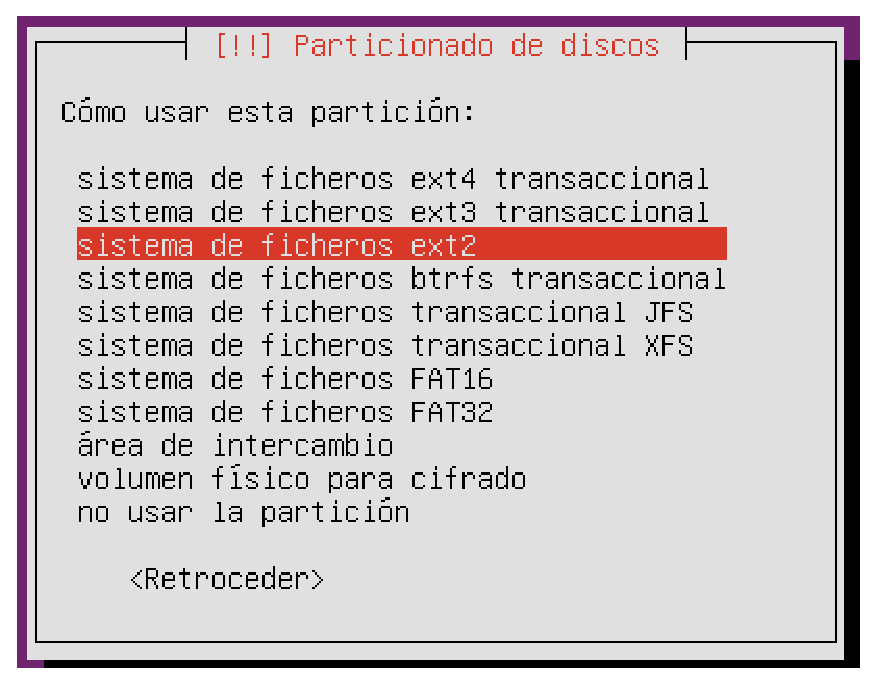
\includegraphics[scale=0.5]{Imagenes/tipos_usos_particiones.eps}
        \caption{Captura de pantalla con los diferentes tipos de uso que el asistente de instalación permite configurar.}
        \label{fig2}
    \end{center}
\end{figure}

Los sitemas de archivos ext4 y ext2, son diferentes versiones de una misma familia de sistemas de archivos,la diferencia entre los dos son las nuevas características añadidas en cada versión, algunas de las nuevas características en ext4 son:\cite{ext} \cite{ext1}
\begin{itemize}
    \item El sistema ext4 puede guardar archivos de 16 TB mientras que ext2 puede hasta 2TB.
    \item En ext4 pueden existir más de  32000 subdirectorios.
    \item Ext4 soporta más de $ 2^{32} $ bloques para el sistema de archivos.
    \item En ext4 pueden existir particiones de hasta 1EB, en ext2 tienen un maximo de 32TB
    \item Ext4 tiene journaling, ext2 no.
\end{itemize}

\subsubsection{Cuestión 12}
\textit{Muestre cómo ha quedado el disco particionado una vez el sistema está instalado. (lsblk)} \newline

El estado final de las particiones es el mostrado en la Figura \ref{fig3}, como se puede ver, todo esta por duplicado ya que es un RAID 1.
\begin{figure}[H]
    \begin{center}
        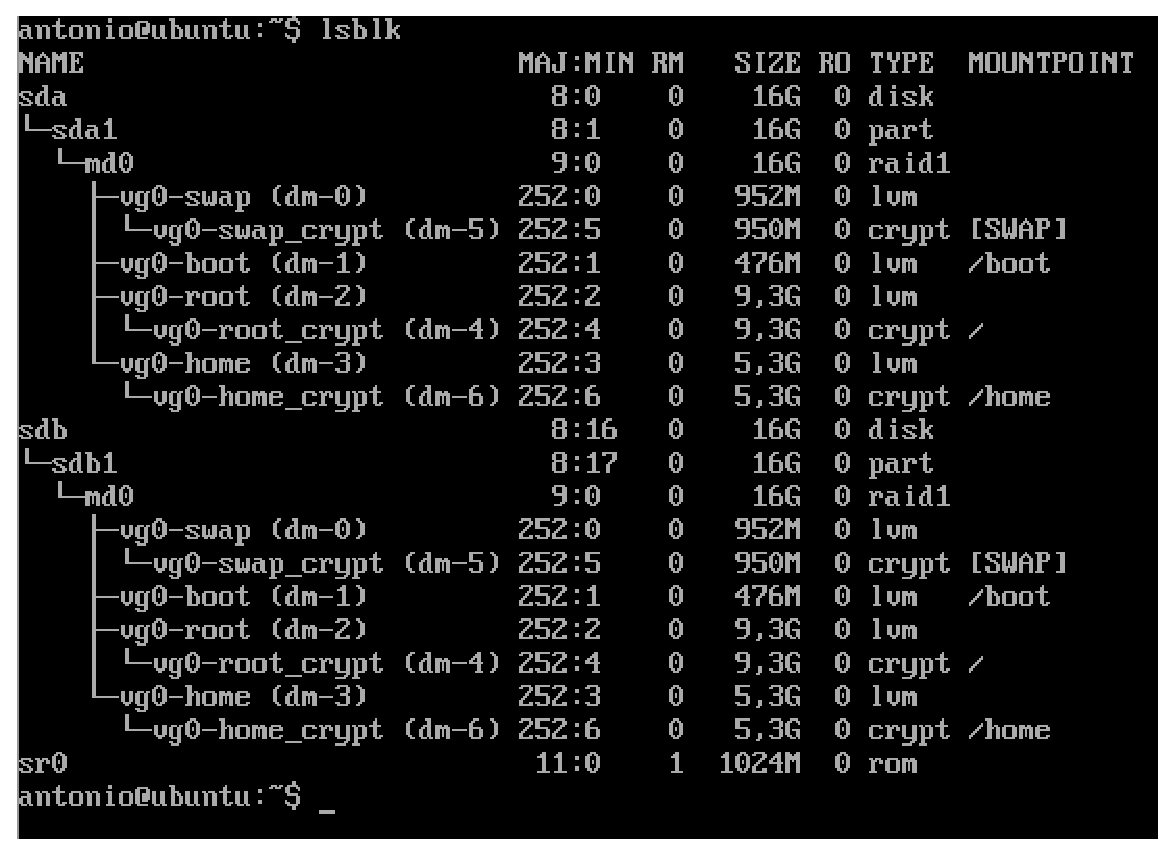
\includegraphics[scale=0.5]{Imagenes/particionado.eps}
        \caption{Estado final de las particiones creadas en el disco.}
        \label{fig3}
    \end{center}
\end{figure}
\subsubsection{Cuestión 13}

\textit{a) ¿Cómo ha hecho el disco 2 “arrancable”? b) ¿Qué hace el comando grub-install? c) ¿Qué hace el comando dd?} \newline
\begin{enumerate}[a)]
    \item Para hacer el disco 2 arrancable he usado la orden \texttt{sudo grub-install /dev/sdb }con la que se consigue instalar GRUB en el MBR de sdb.
    \item El comando grub-install, instala GRUB (GRand Unified Bootloader) en un disco. \cite{grub}
    \item dd es un comando que copia un fichero de entrada en uno de salida, además puede realizar conversiones mediante la especificación de un tamaño de bloque de entrada y un tamaño de bloque de salida. \cite{dd}
\end{enumerate}

\subsubsection{Cuestión opcional 1}
\textit{Muestre (con capturas de pantalla) cómo ha comprobado que el RAID1 funciona.} \newline

La comprobación de que el RAID 1 funciona, se puede llevar a cabo de dos formas, simulando un fallo hardware mediante software o provocando un fallo hardware real.

\begin{description}
    \item[Comprobación simulando fallo mediante software:\cite{pruebaraid}] 
    
 En este caso primero simulamos un fallo de disco (Figura \ref{fig4} ) y vemos que el sistema  sigue funcionado correctamente, por lo que el RAID  está funcionando. Para asegurarnos miramos el estado del disco para comprobar que realmente ha fallado( Figura \ref{fig5} ) y por ultimo, como se puede ver en las Figuras \ref{fig6} y \ref{fig7}, eliminamos el disco que ha fallado y añadimos uno nuevo y comprobamos que el RAID se recupera correctamente ( Figura \ref{fig8} ).

                \begin{figure}[H]
                    \begin{center}
                        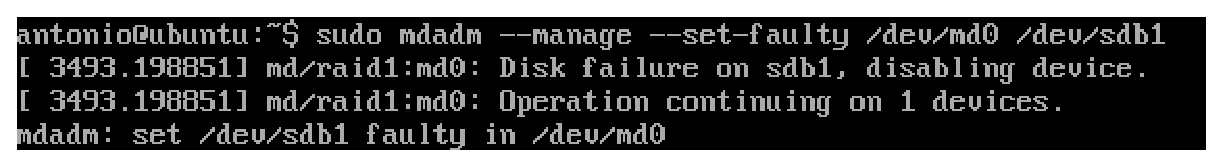
\includegraphics[scale=0.6]{Imagenes/fallo.eps}
                        \caption{Comando para provocar un fallo.}
                        \label{fig4}
                    \end{center}
                \end{figure}

            \begin{figure}[H]
                \begin{center}
                    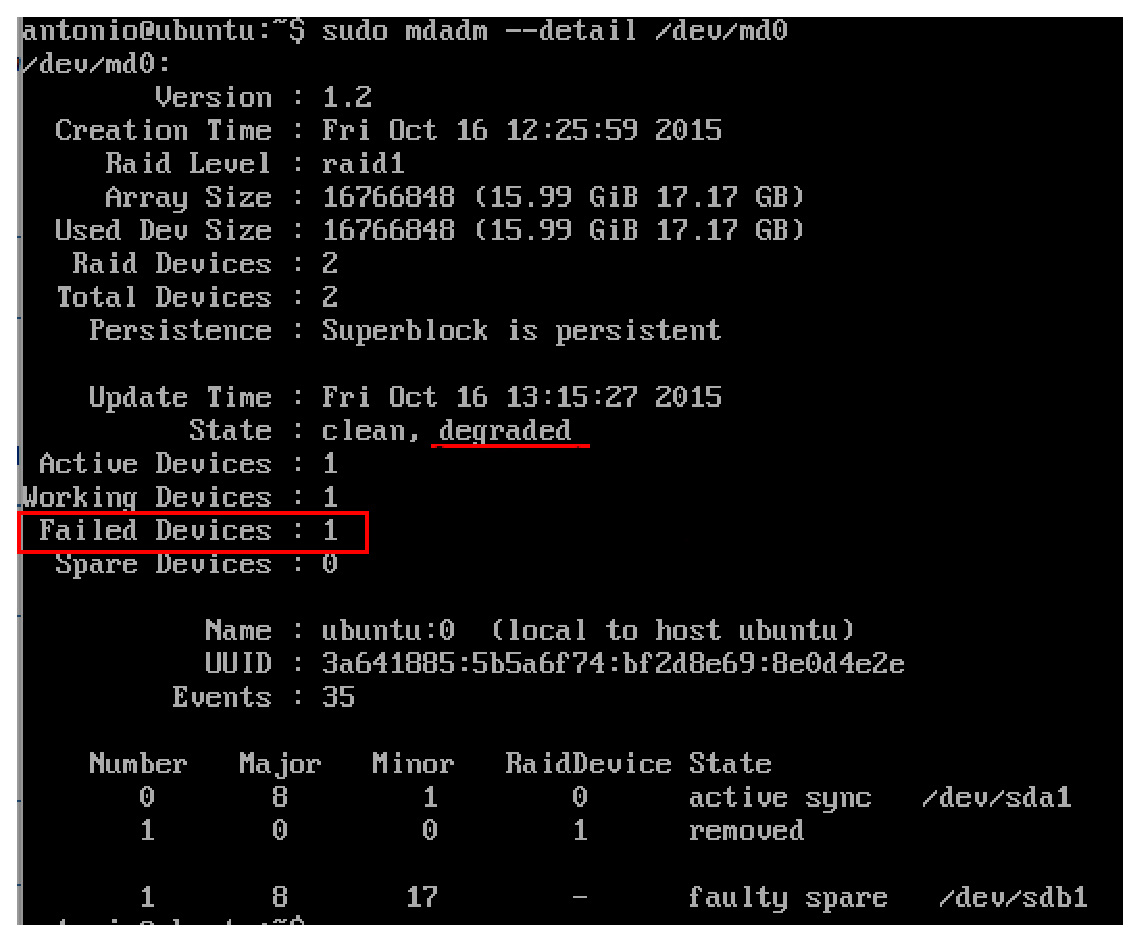
\includegraphics[scale=0.5]{Imagenes/estado_fallo.eps}
                    \caption{Comprobación del estado del RAID.}
                    \label{fig5}
                \end{center}
            \end{figure}

            \begin{figure}[H]
                \begin{center}
                    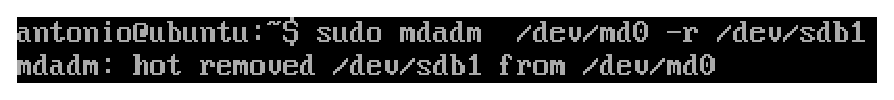
\includegraphics[scale=0.8]{Imagenes/remove.eps}
                    \caption{Eliminación del disco que ha fallado.}
                    \label{fig6}
                \end{center}
            \end{figure}

            \begin{figure}[H]
                \begin{center}
                    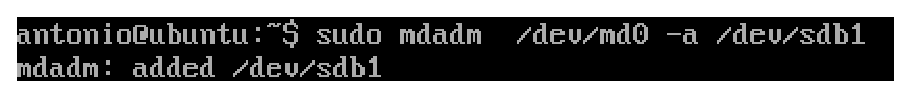
\includegraphics[scale=0.8]{Imagenes/add.eps}
                    \caption{Adición de un disco.}
                    \label{fig7}
                \end{center}
            \end{figure}

            \begin{figure}[H]
                \begin{center}
                    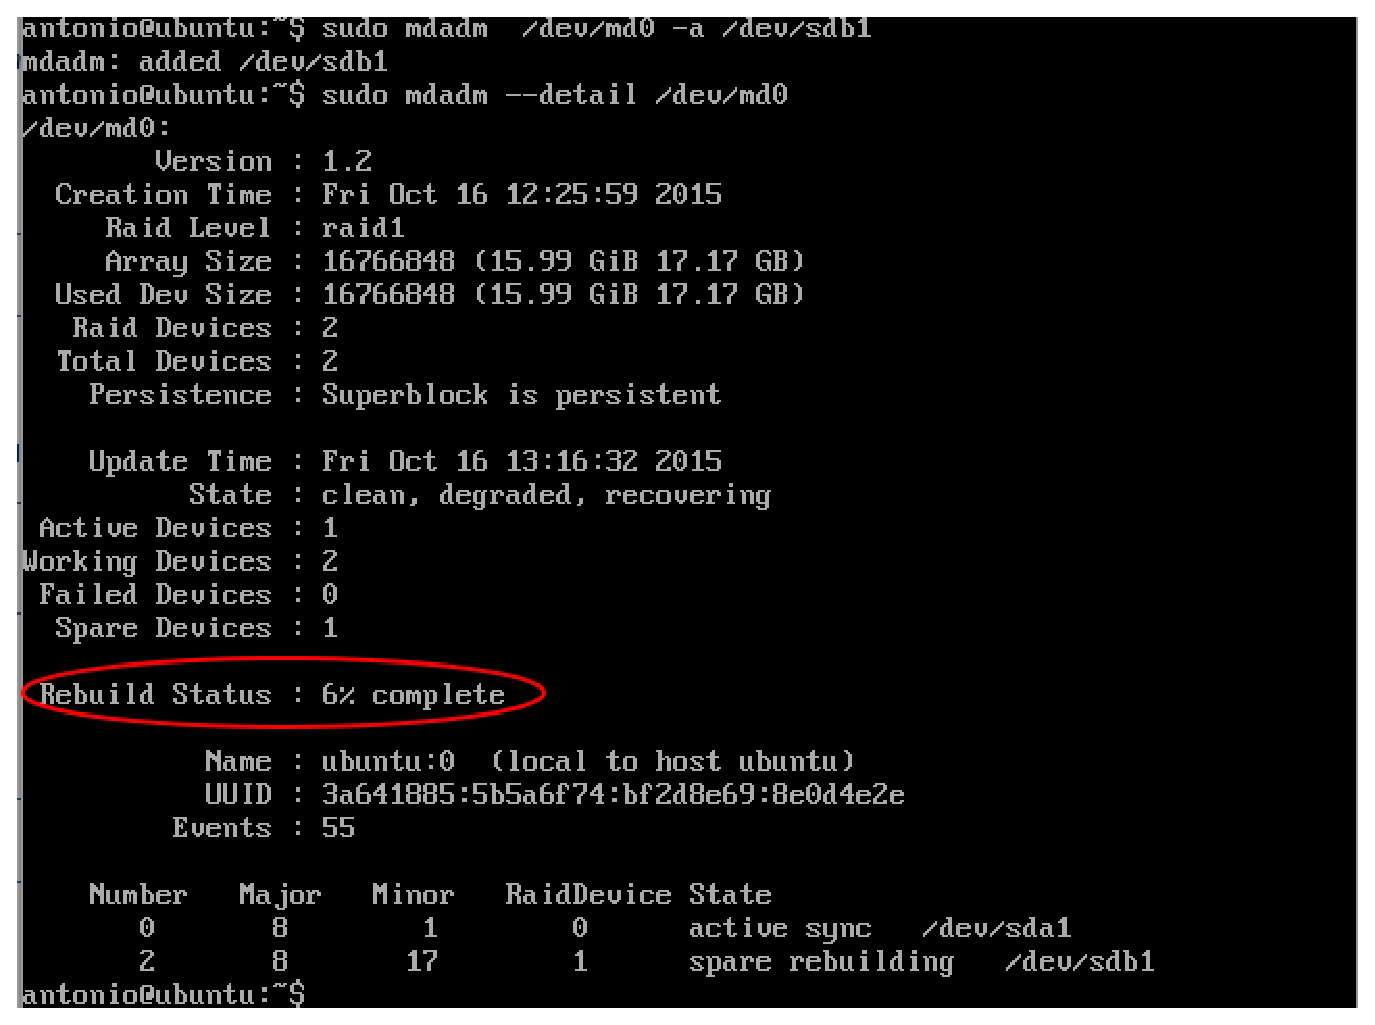
\includegraphics[scale=0.5]{Imagenes/estado_recuperacion.eps}
                    \caption{Comprobación del estado de recuperación del RAID.}
                    \label{fig8}
                \end{center}
            \end{figure}
    \item[Comprobación mediante fallo hardware: ]
    
 Esta comprobación consiste en eliminar un disco del la maquina como se puede ver en el Figura \ref{fig9} y comprobar que el sistema arranca sin problemas. Para que el sistema arranque hay que solucionar un problema de Ubuntu como se indica en el anexo A.1(\nameref{praid}), luego el sistema debe iniciar normalmente y por lo tanto el RAID 1 funciona correctamente. Otra forma de probarlo es quitar un disco mientras que la maquina se esta ejecutando, con lo que se obtendría algo muy similar a lo mostrado en la prueba por software.
            \begin{figure}[H]
                \begin{center}
                    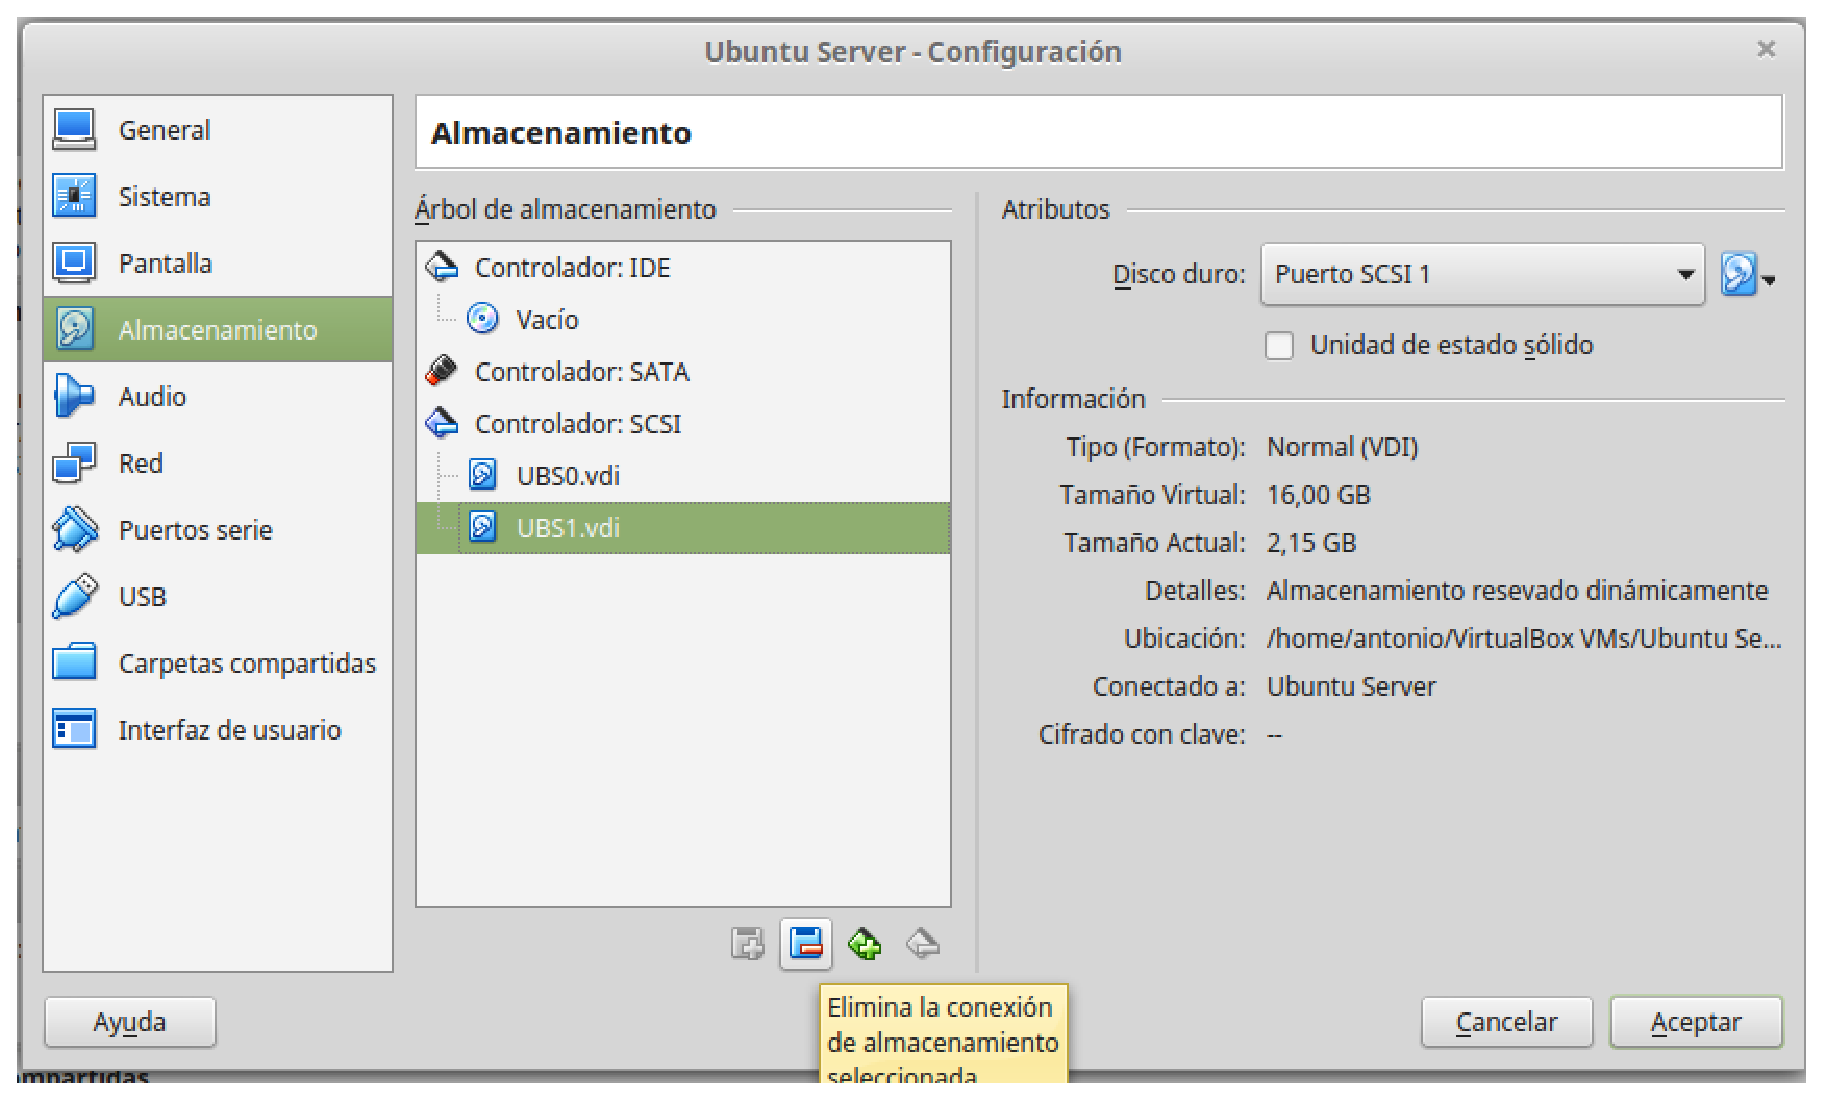
\includegraphics[scale=0.4]{Imagenes/eliminar_disco.eps}
                    \caption{Eliminación de disco en VirtualBox.}
                    \label{fig9}
                \end{center}
            \end{figure}
\end{description}


%*************************************************************
\subsection{Windows Server}
\subsubsection{Cuestión 14}
\textit{¿Qué diferencia hay entre Standard y Datacenter?}\newline

La única diferencia que existe entre la versión standard y la datacenter, es el numero de maquinas virtuales que se pueden ejecutar. La licencia de la versión standard permite tener un máximo de 2 maquinas virtuales, mientras que la versión datacenter no tiene ningún limite, se pueden tener todas las maquinas virtuales que se quieran(dentro de las limitaciones del hardware). \cite{difsd}

\subsubsection{Cuestión 15}
\textit{Continúe usted con el proceso de definición de RAID1 para los dos discos de 50MiB que ha creado. Muestre el proceso con capturas de pantalla.}\newline

La creación de un RAID1 en Windows Server 2008R2 es bastante simple, ya que básicamente la tarea consiste en seguir los pasos del asistente para crear un volumen reflejado, que es lo mismo que un RAID1.Los pasos mas importantes seguidos para la creación del RAID son los mostrados en las siguientes figuras.

\begin{figure}[H]
    \begin{center}
    \advance\leftskip-2.3cm
        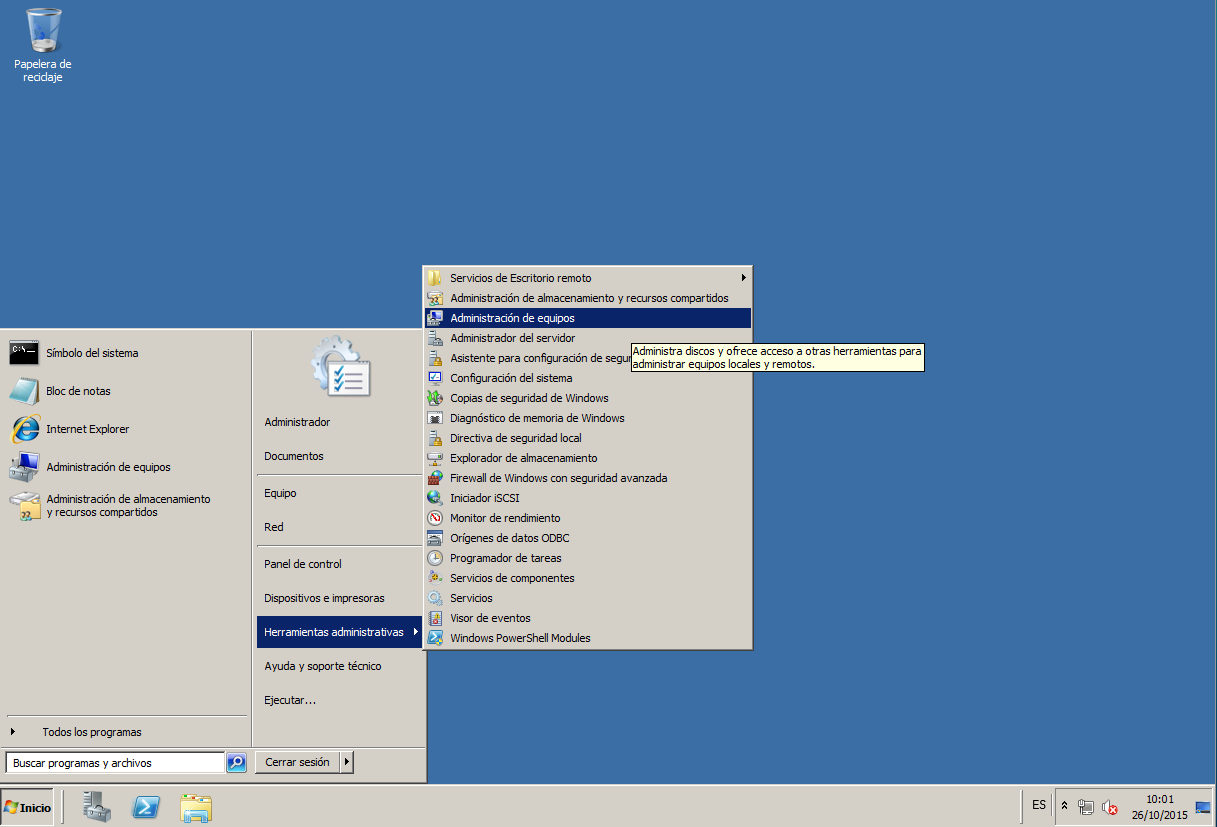
\includegraphics[scale=0.45]{Imagenes/paso1.eps}
        \caption{Acceso al menú de administración de equipos.}
        \label{fig10}
    \end{center}
\end{figure}

\begin{figure}[H]
    \begin{center}
    \advance\leftskip-2cm
        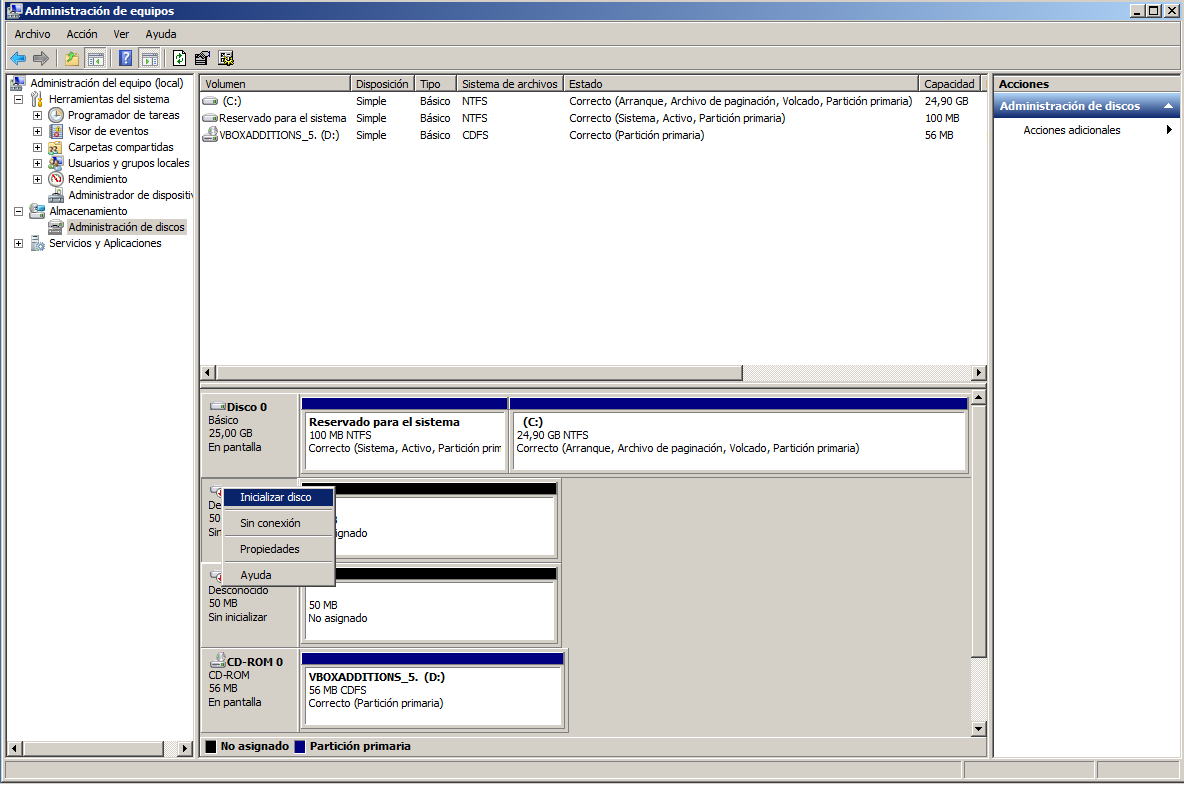
\includegraphics[scale=0.45]{Imagenes/paso2.eps}
        \caption{Inicializar discos en el menú de administración de discos.}
        \label{fig11}
    \end{center}
\end{figure}

\begin{figure}[H]
    \begin{center}
        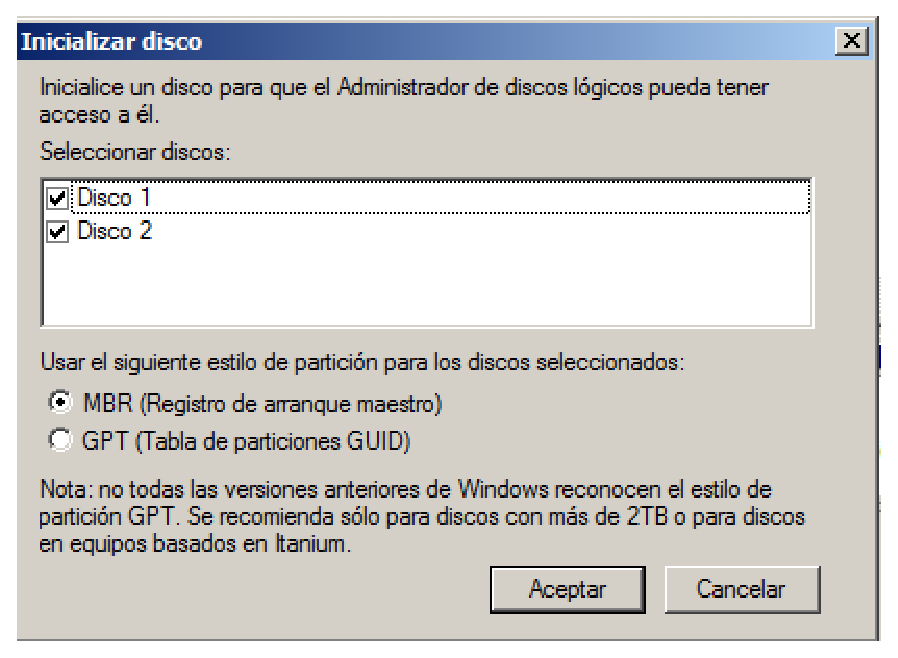
\includegraphics[scale=0.7]{Imagenes/paso3.eps}
        \caption{Seleccionar discos que se desean inicializar.}
        \label{fig12}
    \end{center}
\end{figure}

\begin{figure}[H]
    \begin{center}
        \advance\leftskip-2.1cm
        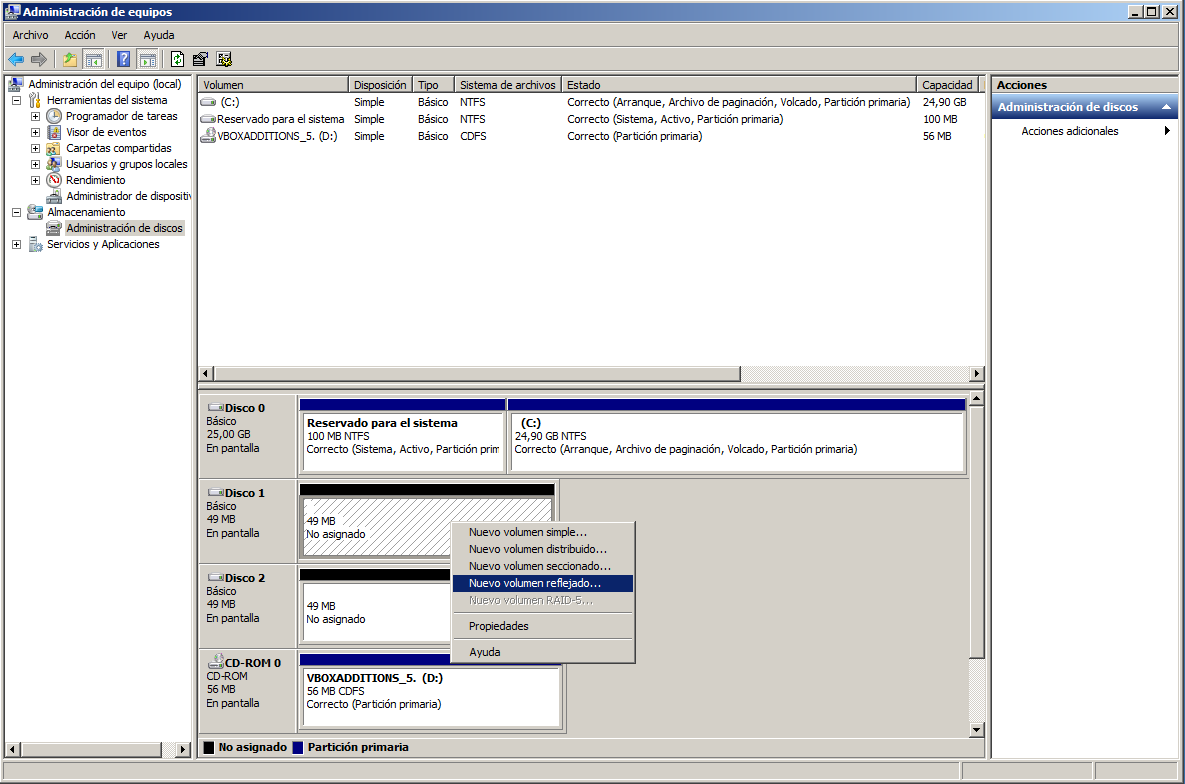
\includegraphics[scale=0.45]{Imagenes/paso4.eps}
        \caption{Creacion de un nuevo volumen reflejado (RAID1) }
        \label{fig13}
    \end{center}
\end{figure}

\begin{figure}[H]
    \begin{center}
        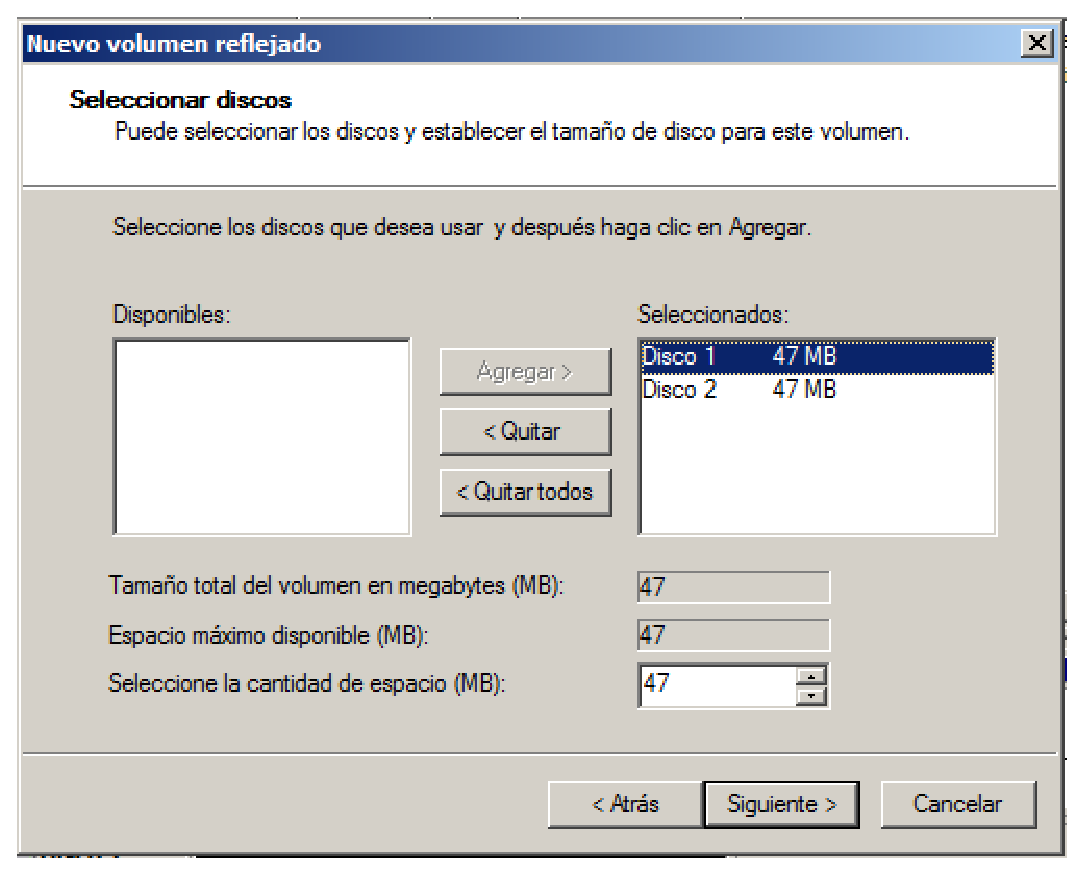
\includegraphics[scale=0.6]{Imagenes/paso5.eps}
        \caption{Seleccionar los discos que se quieren usar para el RAID1.}
        \label{fig14}
    \end{center}
\end{figure}

\begin{figure}[H]
    \begin{center}
        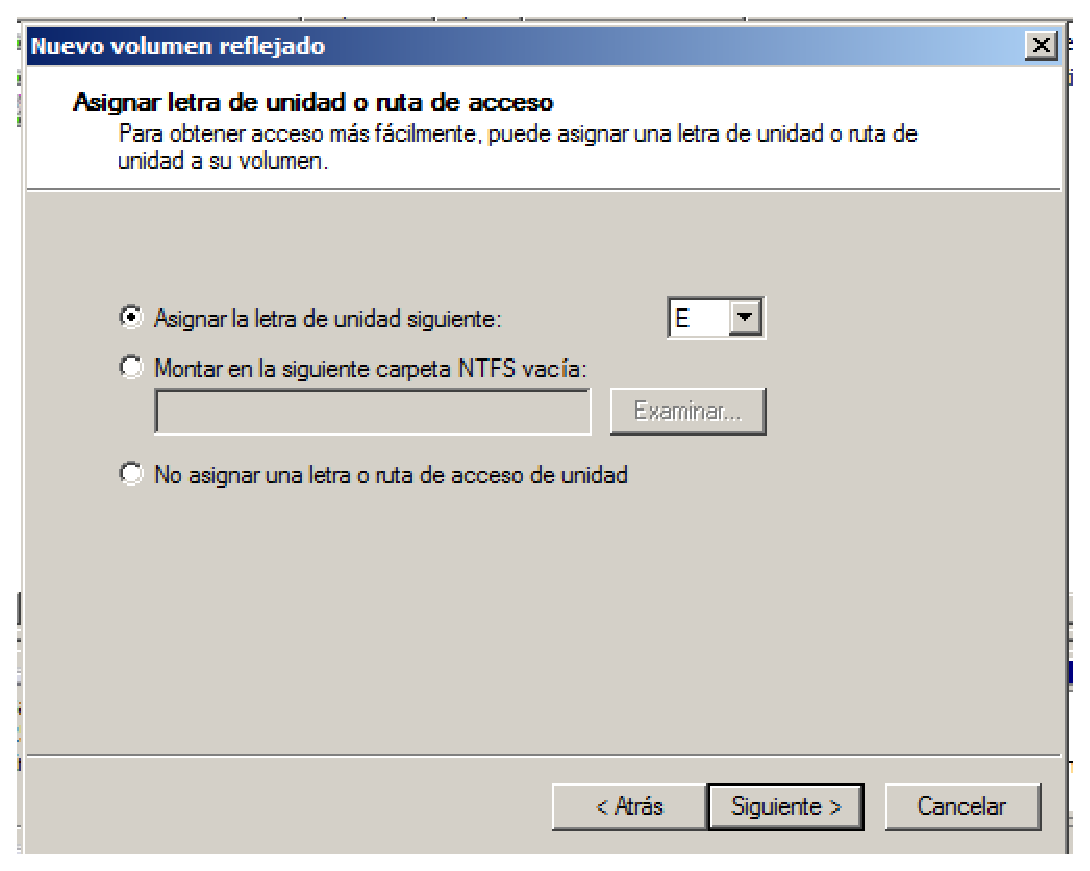
\includegraphics[scale=0.6]{Imagenes/paso6.eps}
        \caption{Asignar una letra al nuevo volumen.}
        \label{fig15}
    \end{center}
\end{figure}

\begin{figure}[H]
    \begin{center}
        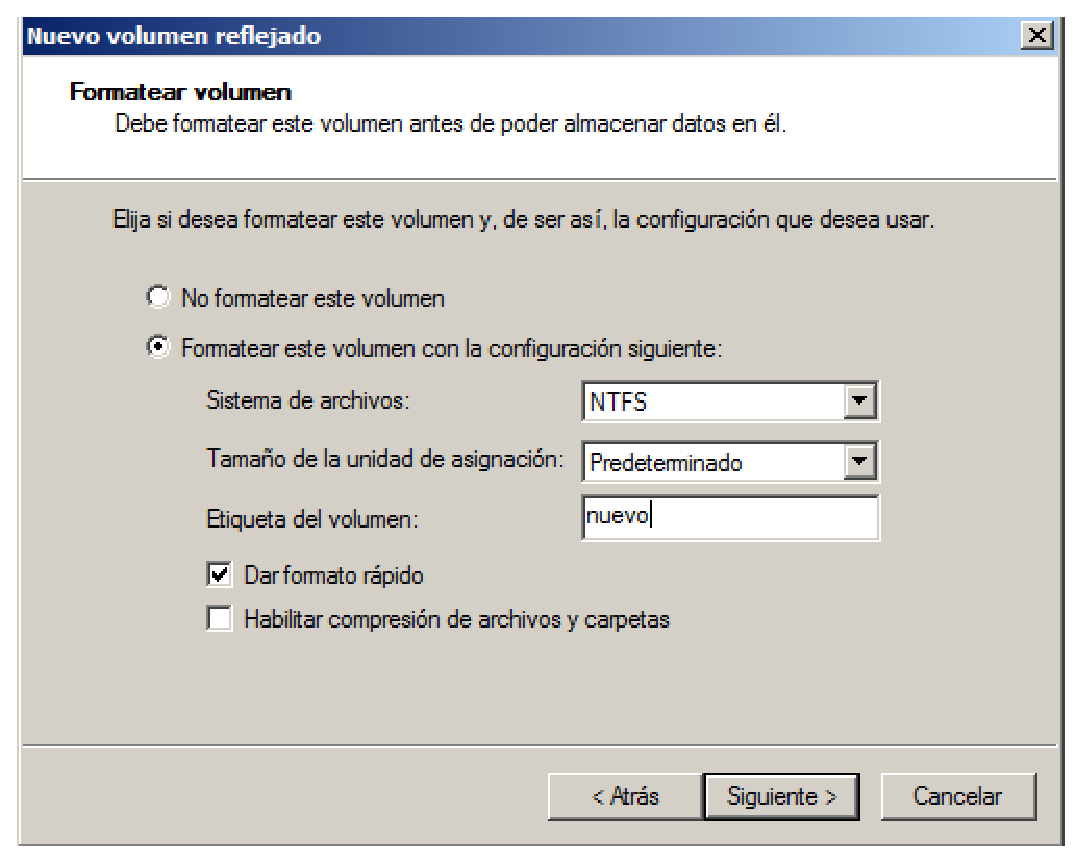
\includegraphics[scale=0.6]{Imagenes/paso7.eps}
        \caption{Opciones de formateo para el nuevo volumen.}
        \label{fig16}
    \end{center}
\end{figure}

\begin{figure}[H]
    \begin{center}
        \advance\leftskip-2.1cm
        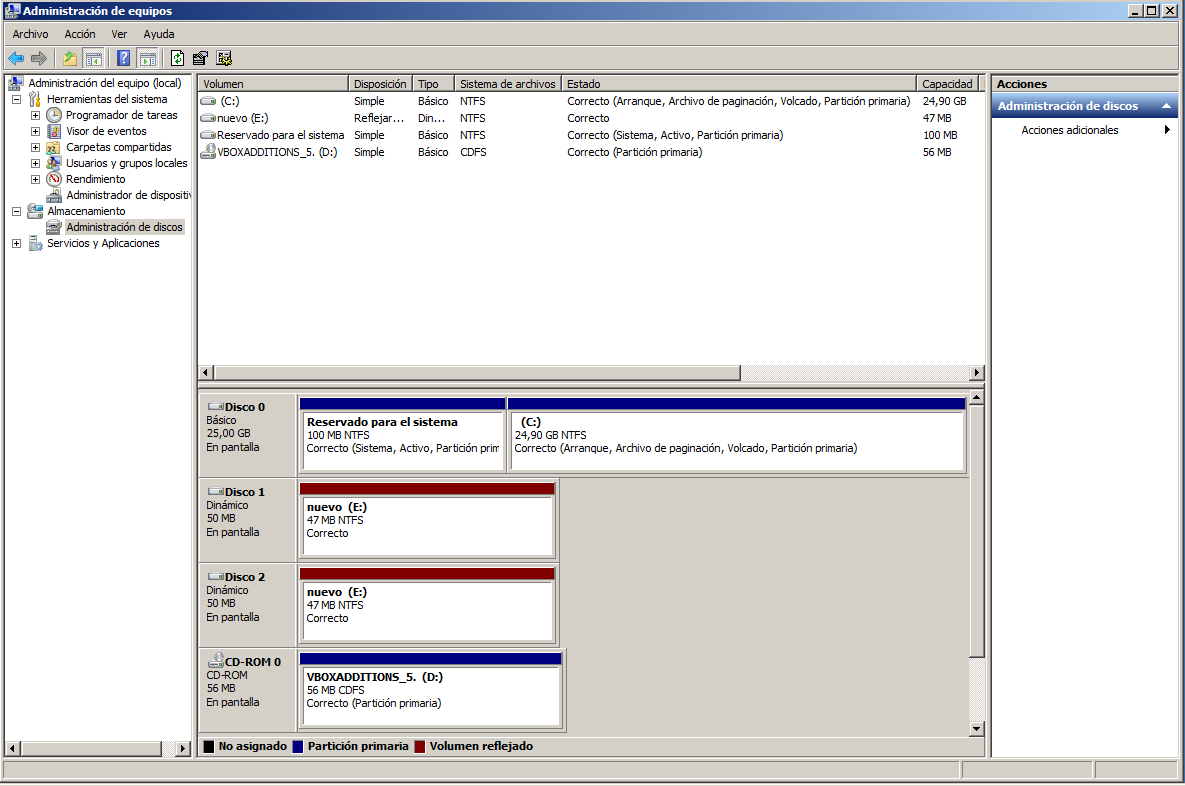
\includegraphics[scale=0.45]{Imagenes/final.eps}
        \caption{Resultado final tras la creación del RAID1.}
        \label{fig17}
    \end{center}
\end{figure}

%*************************************************************
\subsection{Ajuste de parámetros de la máquina virtual}
\subsubsection{Cuestión 16}
\textit{Explique brevemente qué diferencias hay entre los tres tipos de conexión que permite el VMSW para las Mvs: NAT, Host-only y Bridge.}\newline

La conexión bridge conecta la maquina virtual a internet a través de un adaptador de red creado en la maquina host, la maquina tiene una ip visible en el resto de la red local , el tipo de conexión NAT es igual que de conexiones a internet que se tienen en las casas, las maquinas virtuales disponen de una ip privada y pueden acceder a internet y a la red local a través de la maquina host, que hace de router. La red de tipo host-only, crea un red que está dentro del host, que permite conectar la maquina virtual al host, mediante un adaptador de red virtual, en este tipo de conexión, la maquina está aislada del exterior, no puede acceder a internet ni a la red local. \cite{red}

%*************************************************************
\section{Editores de texto}
\subsection{Cuestión opcional 2}
\textit{¿Qué relación hay entre los atajos de teclado de emacs y los de la consola bash? ¿y entre los de vi y las páginas del manual?}\newline
 
 La relación entre los atajos de teclado de emacs y bash, es que la edición de línea de comando (Command Line Editing) viene configurada por defecto con el estilo de emacs \cite{bash1}, aunque es posible cambiarlo al estilo de vi mediante la orden \texttt{set -o vi} \cite{bash2}. 
 
Del segundo apartado de la pregunta no he conseguido obtener ninguna información.
 
 
%*************************************************************


\clearpage
\addappheadtotoc
\appendixpage

\appendix


\section{Solución problemas Ubuntu Server }
\subsection{Problema RAID 1 al desconectar un disco.}
Cuando sacamos por pimera vez un disco del RAID, el dispositivo md se desactiva, para solucionar esto deberemos seguir los siguientes pasos:
En primer lugar iniciamos la maquina virtual y llegara un momento en el que ponga ``waiting for encrypted source device'' (Figura \ref{fig10}) una vez ahí, debemos esperar unos 3 minutos hasta que aparece el promt de initframfs.
Una vez llegados a este punto ejecutamos la orden: \texttt{ cat /proc/mdstat } y podremos ver que el RAID esta desactivado, para solucionarlo ejecutaremos la orden \texttt{mdadm -R /dev/md0}, una vez hecho esto ejecutaremos \texttt{exit} para salir de initramfs y la maquina virtual comenzará a arrancar con normalidad ( Figura \ref{fig11}). \cite{manmdadm}

Tras esto debemos recordar que debemos añadir un nuevo disco al RAID (\texttt{ mdadm /dev/mdX -a /dev/sdXX}) para que vuelva a estar completo.

\begin{figure}[H]
    \begin{center}
        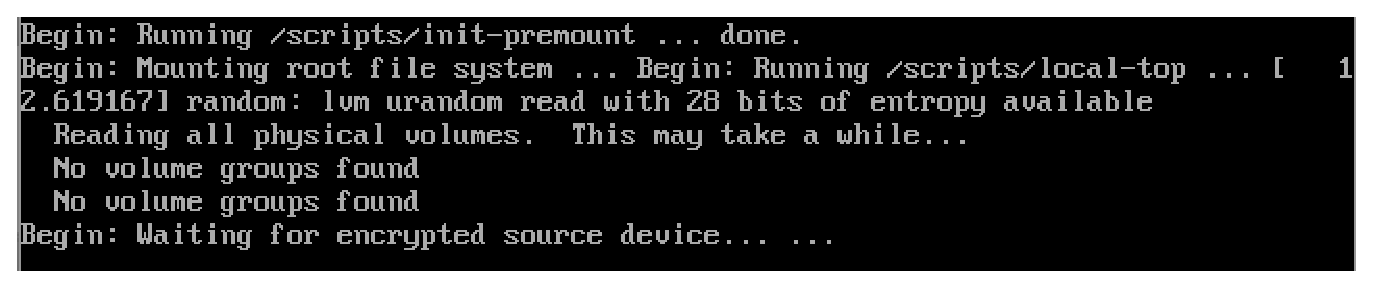
\includegraphics[scale=0.6]{Imagenes/waiting}
        \caption{Mensaje:``waiting for encrypted source device''.}
        \label{fig10}
    \end{center}
\end{figure}

\begin{figure}[H]
    \begin{center}
        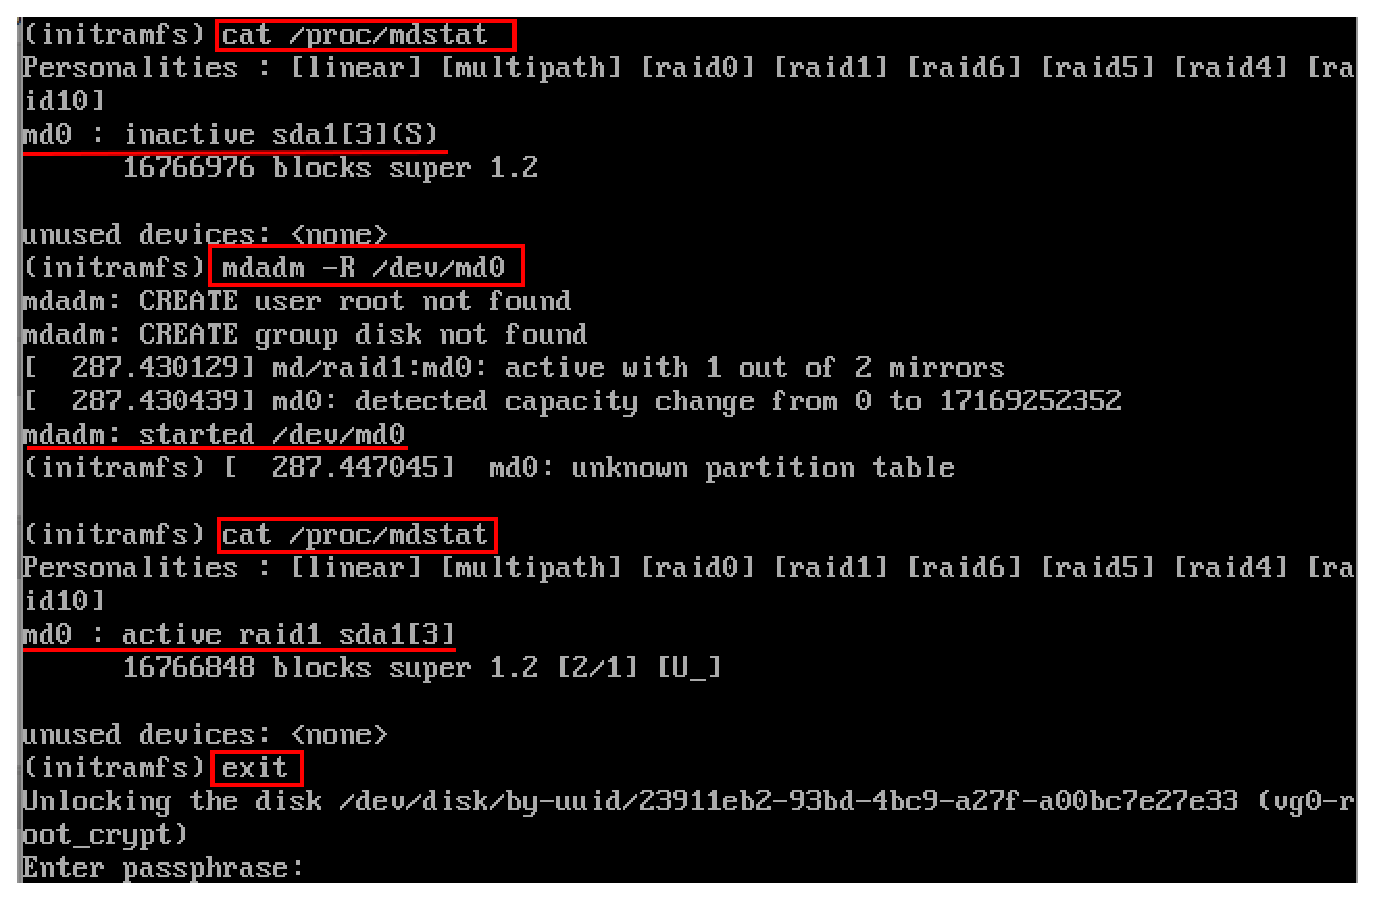
\includegraphics[scale=0.5]{Imagenes/activar}
        \caption{Proceso para arreglar el RAID.}
        \label{fig11}
    \end{center}
\end{figure}


\label{praid}
\subsection{error:  Diskfilter writes are not supported}
Este error es un bug de Ubuntu, que se puede solucionar con el procefimiento indicado en: \href{http://askubuntu.com/questions/468466/why-this-occurs-error-diskfilter-writes-are-not-supported/468487#468487}{boot - Why this occurs error: Diskfilter writes are not supported - Ask Ubuntu}


\newpage
\bibliographystyle{ieeetr}
\bibliography{citas} 

\end{document}
